\section{Methodes d'analyse statistique}

Au cours de ce laboratoire, il vous faudra analyser les données que vous aurez recueillies. Pour cela, vous aurez à votre disposition plusieurs iPython Notebook que vous étudierez en profondeur lors du cours de statistique. Ces différents outils sont accessibles via le lien suivant:\\
\url{https://github.com/zemrude/PHYS-F-311}

\subsection{Méthode Monte Carlo}
Afin de développer votre méthode d'ajustement, il vous sera demandé, dans un premier temps,  de créer un ensemble de données que vous générerez via la technique de simulation Monte Carlo (MC). Vous avez à votre disposition deux méthodes pour générer vos données: la transformation inverse et le "Hit and Miss". A l'aide de ces deux techniques, vous serez en mesure de générer des évènements aléatoires qui suivront la distribution de votre choix (gaussienne, loi exponentielle, ...).

\subsubsection{Hit $\&$ Miss}
La méthode Hit $\&$ Miss ou méthode du rejet consiste à générer aléatoirement un grand nombre d'évènements et à ne sélectionner ensuite que ceux remplissant les conditions pré-établies, i.e. les évènements sous la courbe de la distribution choisie. 

\begin{figure}[h!]
\center{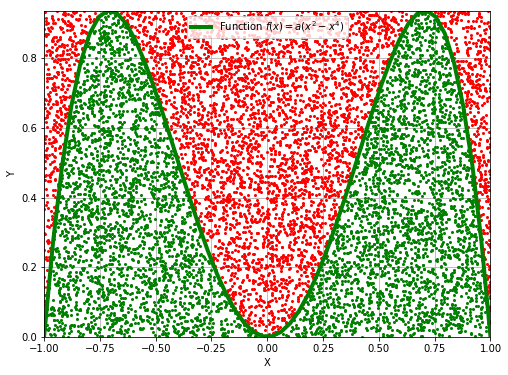
\includegraphics[width=0.6\textwidth]{figures/Hit_and_miss.png}}
\caption{Simulation obtenue par la méthode du Hit $\&$ Miss. Les points représentent les évènements générés aléatoirement. Les éléments en vert sont ceux qui ont remplissent la condition fixée pour suivre la distribution souhaitée. Les points rouges sont rejetés et auront donc été simulés en vain.}
\label{fig:HitMiss}
\end{figure}

Pour notre exemple, la fonction $f(x)=a(x^{2}-x^{4})$ a été choisie. La figure \ref{fig:HitMiss} illustre la méthode du Hit $\&$ Miss en indiquant en vert les points qui sont sous la courbe de la distribution que l'on souhaite reproduire. Les points rouges seront rejetés. Cette méthode demande donc plus de ressources afin d'obtenir suffisamment de statistique puisqu'une partie des évènements générés ne  sera finalement pas utilisée.

\subsubsection{Transformation inverse}
A l'aide de cette méthode,  un échantillon aléatoire de nombres suivant une distribution donnée peut être directement produit. Les données aléatoires sont obtenues à partir de l'inverse de la fonction de répartition. Cette méthode se base sur le théorème de la réciproque. Dans un premier temps, il nous faut calculer l'inverse de notre fonction, $F(x)$, en fonction de $x$. Les évènements générés aléatoirement seront ensuite passé dans la fonction inverse afin d'obtenir la distribution souhaitée. 

\begin{figure}[h!]
\center{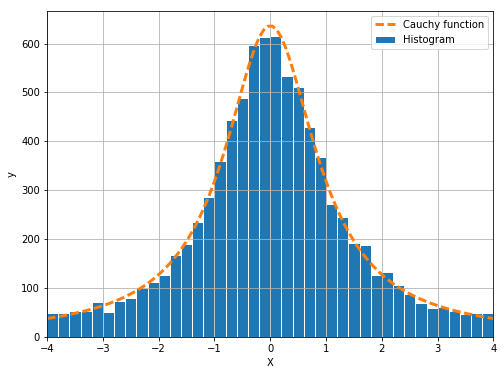
\includegraphics[width=0.6\linewidth]{figures/Inverse_transformation.png}}
\caption{Histogramme des évènements générés par la méthode de transformation inverse pour la distribution de Cauchy.}
\label{fig:Inverse}
\end{figure}

Pour notre exemple illustré par le graphique \ref{fig:Inverse}, nous allons considérer la loi de Cauchy, dont la fonction de répartition s'écrit:

\begin{equation}
F(x) = \frac{1}{2} + \frac{1}{\pi} \arctan \left(\frac{x - x_{0}}{a}\right) \, .
\end{equation}

On a alors:

\begin{equation}
u = F(x) \Longleftrightarrow x = x_{0} + a \tan \left[ \pi  \left(u - \frac{1}{2} \right)  \right] \, .
\end{equation}

La simulation peut donc être obtenue en suivant :

\begin{equation}
X = x_{0} + a \tan \left[ \pi  \left(U - \frac{1}{2} \right)  \right] \, .
\end{equation}

La fonction de Cauchy est indiquée en orange alors que les données simulées obtenues à partir de notre méthode inverse sont mise en histogramme. On peut voir que la distribution de ces évènements reproduit correctement la loi de Cauchy.

\subsection{Ajustement}
Nous allons à présent développer la méthode d'ajustement sur les données que vous venez d'obtenir par la méthode Monte Carlo de votre choix. Deux méthodes vous sont à nouveau proposées pour ce "fit": la méthode des moindre carré ($\chi^2$) et la méthode du maximum de vraisemblance. Ces deux méthodes permettent de comparer nos données avec les prédictions théoriques de notre modèle. Une fois au point, vous pourrez donc utiliser cet ajustement sur vos données réelles afin de vérifier si votre échantillon a bien le comportement attendu. 

\textbf{Remarque :} La minimisation n'est pas effectuée directement sur les données mais sur les données déjà représentées en histogramme.

\subsubsection{Moindre carré - $\chi^{2}$}
Considérons la distribution de nos évènements générés par MC  que l'on désire ajuster au mieux par une fonction $f(x)$ que choisie de manière pertinente en fonction du phénomène étudier. Nous cherchons les paramètres de cette fonction qui minimisent la somme des carrés des distances entre la hauteur de nos barres d'histogrammes, $y_i$, en $x_i$ et $f(x_i)$, autrement dit:

\begin{equation}
\chi^2 = \sum_{i=1}^{N} \left[ y_i - f(x_i) \right]^2 \, .
\end{equation}

Pour notre exemple, nous considérons une distribution d'évènements suivant une décroissance exponentielle dont nous tentons de trouver le temps de vie, $\tau$. Notre fonction est donc donnée par:

\begin{equation}
f(x) = \alpha \exp(-x / \tau) \, .
\end{equation}

La valeur de $\tau$ minimisant $\chi^2$ est illustrée par la figure \ref{fig:chi2}. Celle-ci est utilisée pour l'ajustement de la figure de droite.

\begin{figure*}[h!]
    \centering
    \begin{minipage}[b]{0.48\linewidth}
    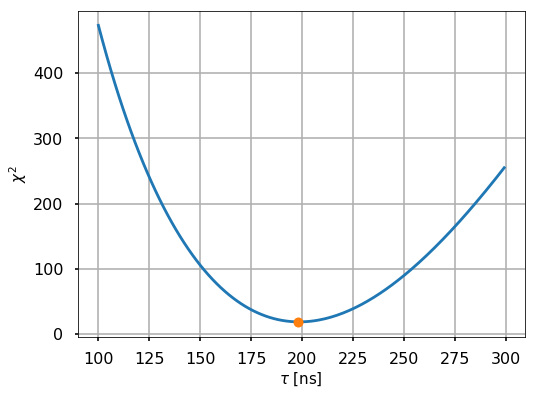
\includegraphics[width=\linewidth]{figures/chi_2.png}
    \end{minipage}
    \hfill
    \begin{minipage}[b]{0.51\linewidth}
    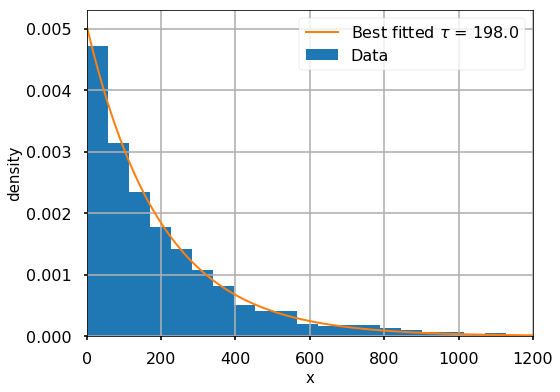
\includegraphics[width=\linewidth]{figures/chi_2_bestfit.png}
    \end{minipage}
    \caption{\textbf{Gauche :} La valeur de $\tau$ minimisant $\chi^2$ est désignée par le point orange. \textbf{Droite :} Le fit obtenu à partir de $\tau_{best}$ (orange) est mis en graphique au côté de la distribution des données MC que nous tentions d'ajuster.}
    \label{fig:chi2}
\end{figure*}

\subsubsection{Maximum de vraisemblance}
La méthode de maximum de vraisemblance est une méthode statistique nous permettant d'évaluer la valeur la plus "vraisemblable" des paramètres d'un modèle probabiliste. 

Pour notre exemple, nous considérons la loi normale exprimée comme suit:

\begin{equation}
f(x) = \frac{1}{\sigma\sqrt{2\pi}} \exp{-\frac{1}{2} \left( \frac{x-\mu}{\sigma}\right)^2} \,  , 
\end{equation}

où $\sigma$ est l'écart type et $\mu$ est la moyenne. Nous allons à présent tenter de trouver la valeur de $\mu$ optimisant la fonction de vraisemblance,  $\mathcal{L}$. Pour cela nous fixons l'écart type de la Gaussienne et laissons varier la moyenne. Nous trouvons ensuite la valeur de $\mu$ qui minimise $-\log{\mathcal{L}}$, comme illustré par la figure \ref{fig:MaxLikelihood}.

\begin{figure*}[h!]
    \centering
    \begin{minipage}[b]{0.49\linewidth}
    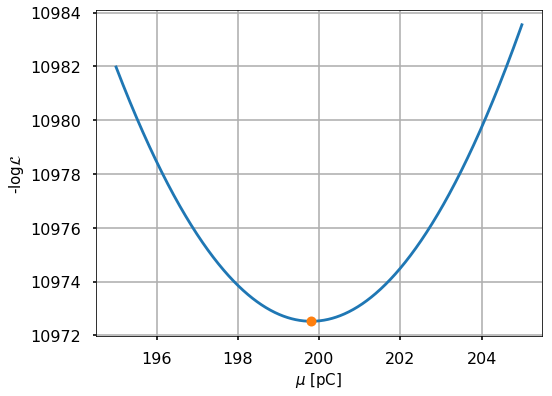
\includegraphics[width=\linewidth]{figures/MaxLikelihood.png}
    \end{minipage}
    \hfill
    \begin{minipage}[b]{0.49\linewidth}
    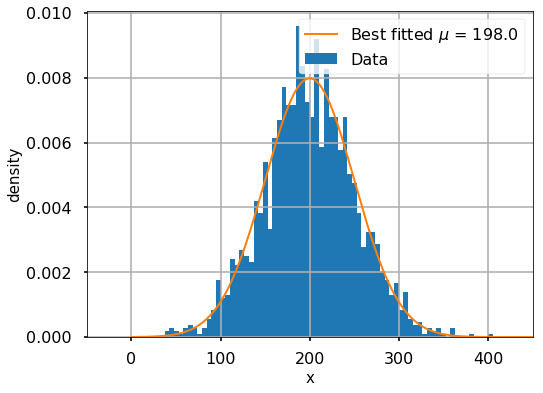
\includegraphics[width=\linewidth]{figures/MaxLikelihood_bestFit.png}
    \end{minipage}
    \caption{\textbf{Gauche :} La valeur de $\mu$ minimisant $-\log{\mathcal{L}}$ est désignée par le point orange. \textbf{Droite :} Le fit obtenu à partir de $\mu_{best}$ (orange) est mis en graphique au côté de la distribution des données MC que nous tentions d'ajuster.}
    \label{fig:MaxLikelihood}
\end{figure*}


\subsection{Erreur sur l'ajustement}
Nous pouvons également estimer l'erreur associée à une valeur ajustée. Nous allons pour cela faire varier de l'unité choisie (1, 2, 3, ...) la valeur minimale de la méthode utilisée. Nous obtiendrons ainsi l'erreur en terme de $\sigma$. L'erreur sur le paramètre à ajuster nous indique alors dans quelle mesure ce paramètre varierait si on répétait le processus de minimisation plusieurs fois.

Pour notre exemple, nous nous intéresseront à la méthode de maximum de vraisemblance. Nous ferons donc varier d'une unité la valeur minimale de  $-\log{\mathcal{L}}$. La barre noire sur le graphique \ref{fig:error} indique l'erreur sur $\mu$ ainsi obtenue.


\begin{figure}[h!]
\center{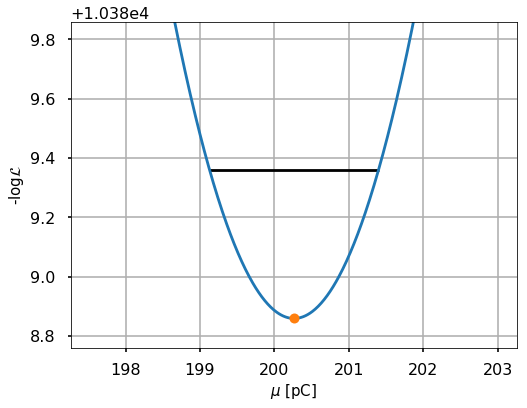
\includegraphics[width=0.6\linewidth]{figures/error.png}}
\caption{Erreur de $1\sigma$ obtenue pour l'exemple précédent de l'ajustement selon la méthode du maximum de vraisemblance.}
\label{fig:error}
\end{figure}




